\documentclass[11pt,a4paper]{article}
\usepackage[margin=1in]{geometry}
\usepackage{amsmath,amssymb}
\usepackage{graphicx}
\usepackage{booktabs}
\usepackage{hyperref}
\usepackage{xcolor}
\usepackage{tikz}
\usetikzlibrary{arrows.meta,positioning,shapes.geometric,fit,backgrounds,calc}
\usepackage{listings}
\usepackage{enumitem}
\usepackage{float}
\usepackage{caption}

\lstset{
  basicstyle=\ttfamily\small,
  backgroundcolor=\color{gray!10},
  frame=single,
  breaklines=true,
  columns=fullflexible,
}

\hypersetup{
  colorlinks=true,
  linkcolor=blue!60!black,
  citecolor=blue!60!black,
  urlcolor=blue!60!black,
}

\title{Mamba-Enhanced GraphCast: Current Method and Setup}
\author{Lianghong Mo}
\date{April 10, 2026}

\begin{document}
\maketitle

\begin{abstract}
This document describes the current implementation of temporal memory in GraphCast using a Mamba selective state space model (SSM). We explain each component from first principles: how GraphCast predicts weather, what Mamba is and how it provides temporal memory, how we combine them via a residual connection, and how we train the combined model using sequential sampling with truncated backpropagation through time (TBPTT). Every parameter is defined with its physical meaning.
\end{abstract}

\tableofcontents
\newpage

%=============================================================================
\section{GraphCast: How It Predicts Weather}
%=============================================================================

\subsection{The Task}

Given the atmospheric state at two consecutive times ($t{-}6\text{h}$ and $t$), predict the state at $t{+}6\text{h}$. The atmospheric state consists of:

\begin{itemize}[nosep]
  \item \textbf{Atmospheric variables} (at each pressure level): temperature, geopotential, u/v wind components, vertical velocity, specific humidity
  \item \textbf{Surface variables}: 2m temperature, 10m u/v wind, mean sea level pressure, 6h precipitation
  \item \textbf{Forcing variables} (known in advance): solar radiation, time-of-year, time-of-day
  \item \textbf{Static variables}: surface geopotential, land-sea mask
\end{itemize}

These are defined on a regular latitude-longitude grid. At resolution 2.0$^\circ$, this is a 91$\times$180 grid (16,380 points). At each grid point, there are 6 atmospheric variables $\times$ 13 pressure levels + 5 surface variables = 83 scalar values per time step.

\subsection{The Pipeline}

GraphCast~\cite{lam2023graphcast} processes one prediction step through four stages:

\begin{figure}[H]
\centering
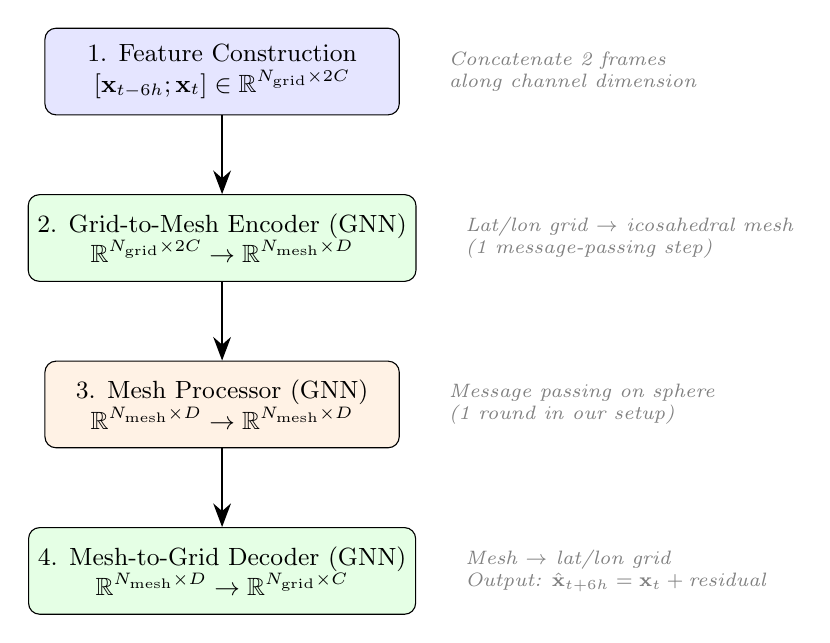
\begin{tikzpicture}[
  box/.style={draw, rounded corners, minimum width=4.5cm, minimum height=1.1cm, align=center, font=\small},
  arrow/.style={-{Stealth[length=3mm]}, thick},
  note/.style={font=\scriptsize\itshape, text=gray, align=left},
]

\node[box, fill=blue!10] (input) {1. Feature Construction\\$[\mathbf{x}_{t-6h}; \mathbf{x}_t] \in \mathbb{R}^{N_\text{grid} \times 2C}$};
\node[box, fill=green!10, below=1.0cm of input] (g2m) {2. Grid-to-Mesh Encoder (GNN)\\$\mathbb{R}^{N_\text{grid} \times 2C} \to \mathbb{R}^{N_\text{mesh} \times D}$};
\node[box, fill=orange!10, below=1.0cm of g2m] (proc) {3. Mesh Processor (GNN)\\$\mathbb{R}^{N_\text{mesh} \times D} \to \mathbb{R}^{N_\text{mesh} \times D}$};
\node[box, fill=green!10, below=1.0cm of proc] (m2g) {4. Mesh-to-Grid Decoder (GNN)\\$\mathbb{R}^{N_\text{mesh} \times D} \to \mathbb{R}^{N_\text{grid} \times C}$};

\draw[arrow] (input) -- (g2m);
\draw[arrow] (g2m) -- (proc);
\draw[arrow] (proc) -- (m2g);

\node[note, right=0.5cm of input] {Concatenate 2 frames\\along channel dimension};
\node[note, right=0.5cm of g2m] {Lat/lon grid $\to$ icosahedral mesh\\(1 message-passing step)};
\node[note, right=0.5cm of proc] {Message passing on sphere\\(1 round in our setup)};
\node[note, right=0.5cm of m2g] {Mesh $\to$ lat/lon grid\\Output: $\hat{\mathbf{x}}_{t+6h} = \mathbf{x}_t + \text{residual}$};

\end{tikzpicture}
\caption{GraphCast pipeline for a single 6-hour prediction step.}
\end{figure}

\subsubsection{Stage 1: Feature Construction}

The two input frames are \textbf{concatenated along the channel dimension}:
\[
\mathbf{f}_i = [\mathbf{x}_{t-6h}^{(i)} \;;\; \mathbf{x}_t^{(i)}] \in \mathbb{R}^{2C}
\]
where $i$ indexes the $N_\text{grid}$ grid points and $C$ is the number of variables per time step. This allows downstream MLPs to learn temporal features like velocity ($\mathbf{x}_t - \mathbf{x}_{t-6h}$) from the concatenated input.

\subsubsection{Stage 2: Grid-to-Mesh Encoder}

A graph neural network maps features from the regular lat/lon grid to an \textbf{icosahedral mesh}---a triangulation of the sphere with approximately uniform node spacing. With \texttt{mesh\_size}$=$4, this mesh has $N_\text{mesh} = 2{,}562$ nodes.

The encoder performs one message-passing step on a bipartite graph (grid nodes $\to$ mesh nodes), producing a mesh latent:
\[
\mathbf{m} \in \mathbb{R}^{N_\text{mesh} \times D}
\]
where $D = 128$ is the latent feature dimension (\texttt{width}).

\subsubsection{Stage 3: Mesh Processor}

The processor runs message passing on the mesh graph. Each mesh node aggregates information from its mesh neighbors:
\[
\mathbf{m}_j^{(k+1)} = \mathbf{m}_j^{(k)} + \text{MLP}\!\left(\mathbf{m}_j^{(k)},\; \textstyle\sum_{j'} \text{MLP}([\mathbf{m}_j^{(k)};\, \mathbf{m}_{j'}^{(k)};\, \mathbf{e}_{jj'}])\right)
\]
In our setup, this runs for 1 round (\texttt{gnn\_msg\_steps}$=$1).

\subsubsection{Stage 4: Mesh-to-Grid Decoder}

A reverse GNN maps mesh features back to the grid. The output is a \textbf{residual} prediction:
\[
\hat{\mathbf{x}}_{t+6h} = \mathbf{x}_t + \text{decode}(\mathbf{m}^{(\text{final})})
\]

\subsection{Multi-Step Forecasting (Autoregressive Rollout)}

For forecasts beyond 6 hours, the prediction is fed back as input:
\[
\underbrace{[\mathbf{x}_{t-6h},\, \mathbf{x}_t]}_{\text{input}} \xrightarrow{\text{predict}} \hat{\mathbf{x}}_{t+6h} \xrightarrow{\text{feed back}} \underbrace{[\mathbf{x}_t,\, \hat{\mathbf{x}}_{t+6h}]}_{\text{new input}} \xrightarrow{\text{predict}} \hat{\mathbf{x}}_{t+12h} \to \cdots
\]

\textbf{The limitation}: Each prediction step sees only the 2 most recent frames. At step $k$, the model has no knowledge of the original initial conditions or any atmospheric state before step $k{-}1$. This is the problem we address with Mamba.

%=============================================================================
\section{Mamba: How It Provides Memory}
%=============================================================================

\subsection{The Selective State Space Model}

Mamba~\cite{gu2023mamba} is a sequence model that maintains a hidden state $h \in \mathbb{R}^H$ which accumulates information over time:
\begin{align}
  h_t &= \underbrace{\bar{A}_t}_{\text{decay}} \cdot\; h_{t-1} \;+\; \underbrace{(1 - \bar{A}_t)}_{\text{update}} \cdot\; u_t \label{eq:state_update}
\end{align}
where:
\begin{itemize}[nosep]
  \item $h_t \in \mathbb{R}^H$ is the hidden state at time $t$ (the ``memory'')
  \item $u_t \in \mathbb{R}^H$ is the projected input at time $t$
  \item $\bar{A}_t = \exp(A \cdot \Delta_t)$ is the \textbf{data-dependent decay} (how much to forget)
  \item $A \in \mathbb{R}^H$ is a learnable log-decay parameter (initialized to $-0.1$)
  \item $\Delta_t = \text{softplus}(\text{Linear}(u_t))$ is the \textbf{data-dependent step size}
\end{itemize}

\textbf{Intuition}: At each time step, the hidden state is a weighted average of the old state and the new input. When $\bar{A}_t \approx 1$ (small $\Delta_t$), the state is mostly preserved (``remember''). When $\bar{A}_t \approx 0$ (large $\Delta_t$), the state is mostly replaced (``forget and update'').

\subsection{The Decay Rate: How Long Is the Memory?}

The parameter \texttt{a\_log} (initialized to $-0.1$) controls the default decay:
\[
A = -\exp(\texttt{a\_log}) = -\exp(-0.1) \approx -0.905
\]
The decay per step is $\bar{A} = \exp(A \cdot \Delta)$. For a typical $\Delta \approx 1$:
\[
\bar{A} \approx \exp(-0.905) \approx 0.40
\]
After $k$ steps without update, the state decays to $\bar{A}^k$:

\begin{center}
\begin{tabular}{ccccccc}
\toprule
Steps & 1 & 3 & 5 & 10 & 20 \\
Time & 6h & 18h & 30h & 2.5d & 5d \\
Remaining & 40\% & 6.5\% & 1.1\% & 0.01\% & $\sim$0\% \\
\bottomrule
\end{tabular}
\end{center}

In practice, $\Delta_t$ is data-dependent and learned, so the effective memory length varies. But the initialization gives the model a starting point of roughly 1--3 steps (6--18 hours) of strong memory.

\subsection{The Full SSM Block}

Our Mamba block takes a mesh latent $\mathbf{m} \in \mathbb{R}^{N_\text{mesh} \times D}$ and produces an output of the same shape:

\begin{enumerate}[nosep]
  \item \textbf{Layer normalization}: $\tilde{\mathbf{m}} = \text{LayerNorm}(\mathbf{m})$
  \item \textbf{Input projection}: $[\mathbf{u},\, \mathbf{g}] = \text{Linear}_{2H}(\tilde{\mathbf{m}})$ \quad (split into value $\mathbf{u}$ and gate $\mathbf{g}$, each $\in \mathbb{R}^H$)
  \item \textbf{Step size}: $\Delta = \text{softplus}(\text{Linear}_H(\mathbf{u}))$ \quad (data-dependent discretization)
  \item \textbf{State update}: $h_\text{new} = \exp(A \cdot \Delta) \cdot h_\text{prev} + (1 - \exp(A \cdot \Delta)) \cdot \mathbf{u}$
  \item \textbf{Gated output}: $\mathbf{y} = h_\text{new} \odot \sigma(\mathbf{g}) + \texttt{skip} \cdot \mathbf{u}$ \quad (sigmoid gating + skip connection)
  \item \textbf{Output projection}: $\Delta\mathbf{m} = \text{Linear}_D(\mathbf{y})$ \quad (project back to mesh latent dimension)
  \item \textbf{Residual}: $\mathbf{m}' = \mathbf{m} + \Delta\mathbf{m}$ \quad (add correction to original)
\end{enumerate}

The residual connection in step 7 is critical: if Mamba learns nothing useful, $\Delta\mathbf{m} \to \mathbf{0}$ and the output equals the input (baseline behavior).

%=============================================================================
\section{Combining GraphCast and Mamba}
%=============================================================================

\subsection{Where Mamba Is Inserted}

We insert the Mamba block \textbf{between the encoder and processor} (location: \texttt{mesh\_post\_encoder\_residual}):

\begin{figure}[H]
\centering
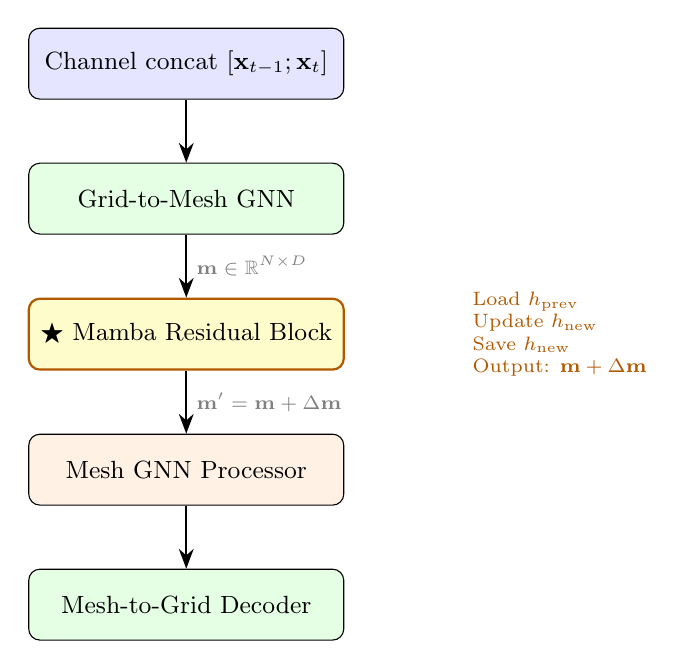
\begin{tikzpicture}[
  box/.style={draw, rounded corners, minimum width=4cm, minimum height=0.9cm, align=center, font=\small},
  mamba/.style={draw, rounded corners, minimum width=4cm, minimum height=0.9cm, align=center, font=\small, fill=yellow!20, draw=orange!70!black, thick},
  arrow/.style={-{Stealth[length=2.5mm]}, thick},
  note/.style={font=\scriptsize\itshape, text=gray},
]

\node[box, fill=blue!10] (input) {Channel concat $[\mathbf{x}_{t-1};\mathbf{x}_t]$};
\node[box, fill=green!10, below=0.8cm of input] (g2m) {Grid-to-Mesh GNN};
\node[mamba, below=0.8cm of g2m] (mamba) {$\bigstar$ Mamba Residual Block};
\node[box, fill=orange!10, below=0.8cm of mamba] (proc) {Mesh GNN Processor};
\node[box, fill=green!10, below=0.8cm of proc] (m2g) {Mesh-to-Grid Decoder};

\draw[arrow] (input) -- (g2m);
\draw[arrow] (g2m) -- (mamba) node[midway, right, note] {$\mathbf{m} \in \mathbb{R}^{N \times D}$};
\draw[arrow] (mamba) -- (proc) node[midway, right, note] {$\mathbf{m}' = \mathbf{m} + \Delta\mathbf{m}$};
\draw[arrow] (proc) -- (m2g);

\node[right=1.5cm of mamba, font=\scriptsize, align=left, text=orange!70!black] {Load $h_\text{prev}$\\Update $h_\text{new}$\\Save $h_\text{new}$\\Output: $\mathbf{m} + \Delta\mathbf{m}$};

\end{tikzpicture}
\caption{Mamba is inserted as a residual block between encoder and processor. Everything above and below it is identical to baseline GraphCast.}
\end{figure}

\textbf{Key design choice}: The encoding path (channel concatenation $\to$ single Grid-to-Mesh pass) is \textbf{identical} to the baseline. Mamba only adds a residual correction. This ensures any performance difference is due to temporal memory, not a different encoding.

\subsection{What Mamba Does at Each Prediction Step}

During autoregressive rollout, Mamba maintains a hidden state $h$ that carries information across prediction steps:

\begin{figure}[H]
\centering
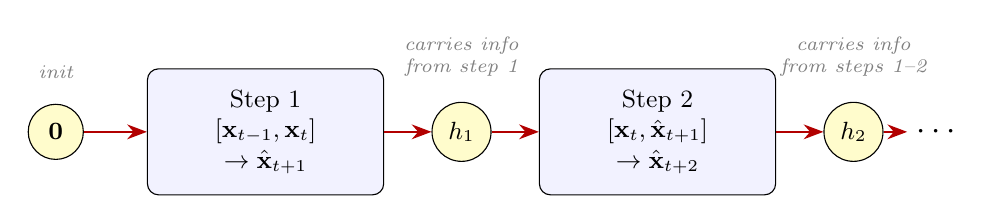
\begin{tikzpicture}[
  rollstep/.style={draw, rounded corners, minimum width=3cm, minimum height=1.6cm, align=center, font=\small, fill=blue!5},
  state/.style={draw, circle, minimum size=0.7cm, font=\small\bfseries, fill=yellow!20},
  arrow/.style={-{Stealth[length=2.5mm]}, thick},
  sarrow/.style={-{Stealth[length=2.5mm]}, thick, color=red!70!black},
]

\node[state] (h0) {$\mathbf{0}$};
\node[rollstep, right=0.8cm of h0] (s1) {Step 1\\$[\mathbf{x}_{t-1}, \mathbf{x}_t]$\\$\to \hat{\mathbf{x}}_{t+1}$};
\node[state, right=0.6cm of s1] (h1) {$h_1$};
\node[rollstep, right=0.6cm of h1] (s2) {Step 2\\$[\mathbf{x}_t, \hat{\mathbf{x}}_{t+1}]$\\$\to \hat{\mathbf{x}}_{t+2}$};
\node[state, right=0.6cm of s2] (h2) {$h_2$};
\node[right=0.3cm of h2, font=\large] (dots) {$\cdots$};

\draw[sarrow] (h0) -- (s1);
\draw[sarrow] (s1) -- (h1);
\draw[sarrow] (h1) -- (s2);
\draw[sarrow] (s2) -- (h2);
\draw[sarrow] (h2) -- (dots);

\node[above=0.2cm of h0, font=\scriptsize\itshape, text=gray] {init};
\node[above=0.2cm of h1, font=\scriptsize\itshape, text=gray, align=center] {carries info\\ from step 1};
\node[above=0.2cm of h2, font=\scriptsize\itshape, text=gray, align=center] {carries info\\ from steps 1--2};

\end{tikzpicture}
\caption{Hidden state $h$ is passed from one prediction step to the next. At step $k$, $h_k$ contains a compressed summary of the forecast trajectory from the initial condition through step $k$.}
\end{figure}

At each step, Mamba:
\begin{enumerate}[nosep]
  \item \textbf{Loads} the hidden state $h_\text{prev}$ from the previous step
  \item \textbf{Reads} the current mesh latent $\mathbf{m}$ (which encodes the current atmospheric state)
  \item \textbf{Updates}: $h_\text{new} = \text{decay} \cdot h_\text{prev} + (1-\text{decay}) \cdot \text{proj}(\mathbf{m})$
  \item \textbf{Outputs} a residual correction: $\Delta\mathbf{m} = f(h_\text{new}, \mathbf{m})$
  \item \textbf{Saves} $h_\text{new}$ for the next step
\end{enumerate}

The baseline model has no equivalent---each prediction step is completely independent.

\subsection{State Shape and Batch Handling}

The hidden state has shape $(N_\text{mesh}, H) = (2562, 128)$, stored \textbf{per mesh node} and \textbf{independent of batch size}. Each mesh node's 128-dimensional state encodes temporal information about the atmospheric evolution at that spatial location.

During training with batch\_size $> 1$, the state is tiled across the batch for the forward pass, then averaged back to $(N_\text{mesh}, H)$ before saving. During inference with batch\_size $= 1$, the state is exact.

%=============================================================================
\section{Training: Sequential Sampling with Truncated BPTT}
%=============================================================================

\subsection{The Problem with Random Sampling}

Standard training draws random time windows from the training data. Each sample is independent (i.i.d.), and the Mamba state is \textbf{reset to zero} before every sample. With \texttt{target\_steps}$=$2, Mamba sees only 1 state transfer per sample---far too little to learn useful temporal patterns.

\subsection{Our Solution: Chunked Sequential Sampling}

We divide the training data into contiguous segments and iterate through them sequentially, carrying the Mamba state forward within each segment:

\begin{figure}[H]
\centering
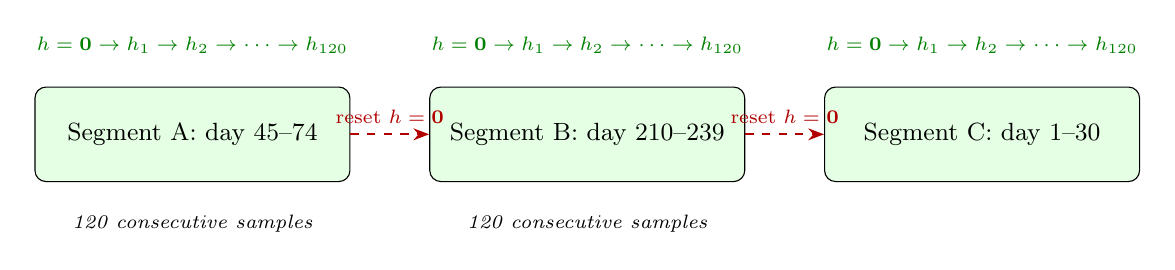
\begin{tikzpicture}[
  seg/.style={draw, rounded corners, minimum width=4cm, minimum height=1.2cm, align=center, font=\small, fill=green!10},
  sample/.style={draw, minimum width=0.6cm, minimum height=0.8cm, fill=blue!10, font=\tiny},
  state/.style={font=\scriptsize, text=red!70!black},
  arrow/.style={-{Stealth[length=2mm]}, thick, color=green!50!black},
  rarrow/.style={-{Stealth[length=2mm]}, thick, color=red!70!black, dashed},
]

\node[seg] (seg1) {Segment A: day 45--74};
\node[seg, right=1cm of seg1] (seg2) {Segment B: day 210--239};
\node[seg, right=1cm of seg2] (seg3) {Segment C: day 1--30};

\node[above=0.3cm of seg1, font=\scriptsize\itshape, text=green!50!black] {$h = \mathbf{0} \to h_1 \to h_2 \to \cdots \to h_{120}$};
\node[above=0.3cm of seg2, font=\scriptsize\itshape, text=green!50!black] {$h = \mathbf{0} \to h_1 \to h_2 \to \cdots \to h_{120}$};
\node[above=0.3cm of seg3, font=\scriptsize\itshape, text=green!50!black] {$h = \mathbf{0} \to h_1 \to h_2 \to \cdots \to h_{120}$};

\draw[rarrow] (seg1) -- (seg2) node[midway, above, font=\scriptsize, text=red!70!black] {reset $h=\mathbf{0}$};
\draw[rarrow] (seg2) -- (seg3) node[midway, above, font=\scriptsize, text=red!70!black] {reset $h=\mathbf{0}$};

\node[below=0.3cm of seg1, font=\scriptsize\itshape] {120 consecutive samples};
\node[below=0.3cm of seg2, font=\scriptsize\itshape] {120 consecutive samples};

\end{tikzpicture}
\caption{Segments are shuffled across epochs. Within each segment, data is sequential and state carries forward. State resets at segment boundaries.}
\end{figure}

\subsection{Step-by-Step Training Procedure}

\begin{enumerate}
  \item \textbf{Segment construction}: Divide the 2020--2021 ERA5 data (2,920 time steps at 6h intervals) into contiguous segments of \texttt{sequential\_segment\_steps}$=$120 steps (30 days). This yields $\sim$24 segments.

  \item \textbf{Epoch start}: Randomly shuffle the order of segments.

  \item \textbf{Segment start}: Reset Mamba state to $\mathbf{0}$.

  \item \textbf{For each consecutive sample within the segment}:
  \begin{enumerate}
    \item \textbf{State handling}:
    \begin{itemize}[nosep]
      \item First sample in segment: $h = \mathbf{0}$ (cold start)
      \item Otherwise: $h = \texttt{stop\_gradient}(h_\text{prev})$ --- state values are preserved but \textbf{gradients are detached}
    \end{itemize}

    \item \textbf{Build training sample}: Extract consecutive window from the data:
    \begin{itemize}[nosep]
      \item Input: $[\mathbf{x}_i, \mathbf{x}_{i+1}]$ (2 frames, 12 hours)
      \item Targets: $[\mathbf{x}_{i+2}, \ldots, \mathbf{x}_{i+1+K}]$ ($K$ = \texttt{target\_steps} future frames)
    \end{itemize}

    \item \textbf{Forward pass}: Run $K$ autoregressive rollout steps through GraphCast + Mamba. At each step, Mamba loads $h$, processes the mesh latent, saves updated $h$.

    \item \textbf{Loss}: $\mathcal{L} = \frac{1}{K}\sum_{k=1}^{K} \text{wMSE}(\hat{\mathbf{x}}_{i+1+k},\; \mathbf{x}_{i+1+k})$

    \item \textbf{Backward pass}: Compute gradients of $\mathcal{L}$ w.r.t.\ all parameters. Gradients flow through the $K$ rollout steps and through the Mamba state chain ($h_K \to h_{K-1} \to \cdots \to h_1$), but \textbf{stop at $h_\text{prev}$} due to \texttt{stop\_gradient}.

    \item \textbf{Parameter update}: Apply AdamW optimizer.

    \item \textbf{Save state}: Store $h_K$ for the next sample.
  \end{enumerate}

  \item \textbf{Segment end}: Move to next segment, reset $h = \mathbf{0}$.

  \item \textbf{Epoch end}: Reshuffle segments, repeat.
\end{enumerate}

\subsection{Truncated BPTT: What Gradients Can and Cannot See}

The \texttt{stop\_gradient} at sample boundaries creates a ``truncation window'' of $K$ steps:

\begin{figure}[H]
\centering
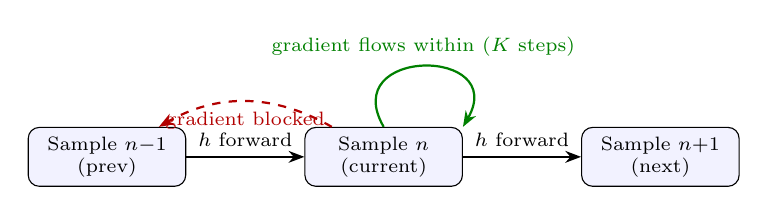
\begin{tikzpicture}[
  node distance=0.8cm,
  sample/.style={draw, rounded corners, minimum width=2cm, minimum height=0.7cm, align=center, font=\scriptsize, fill=blue!5},
  arrow/.style={-{Stealth[length=2mm]}, thick},
  garrow/.style={-{Stealth[length=2mm]}, thick, color=green!50!black},
  sarrow/.style={-{Stealth[length=2mm]}, thick, color=red!70!black, dashed},
]

\node[sample] (s1) {Sample $n{-}1$\\(prev)};
\node[sample, right=1.5cm of s1] (s2) {Sample $n$\\(current)};
\node[sample, right=1.5cm of s2] (s3) {Sample $n{+}1$\\(next)};

\draw[arrow] (s1) -- (s2) node[midway, above, font=\scriptsize] {$h$ forward};
\draw[arrow] (s2) -- (s3) node[midway, above, font=\scriptsize] {$h$ forward};

\draw[sarrow, bend right=30] (s2) to node[below, font=\scriptsize, text=red!70!black] {gradient blocked} (s1);
\draw[garrow, bend left=20] (s2.north) to[out=120,in=60,looseness=3] node[above, font=\scriptsize, text=green!50!black] {gradient flows within ($K$ steps)} (s2.north east);

\end{tikzpicture}
\caption{Forward: state flows across all samples in a segment. Backward: gradient only flows within the current sample's $K$ rollout steps.}
\end{figure}

\textbf{What the model learns}:
\begin{itemize}[nosep]
  \item \textbf{Reading state}: The model learns to extract useful information from $h_\text{prev}$ (which contains accumulated history). This is trained because $h_\text{prev}$ affects predictions within the current sample.
  \item \textbf{Writing state}: The model learns what to store in $h$ that helps predictions 1--$K$ steps later. This is trained through the gradient chain within the sample.
  \item \textbf{Not trained}: How to write state that helps predictions $> K$ steps later. The writing policy is optimized for short-term utility but may naturally produce state that is also useful long-term (due to the SSM decay dynamics).
\end{itemize}

%=============================================================================
\section{Inference Procedure}
%=============================================================================

At inference time, the model receives an initial condition and rolls out freely:

\begin{enumerate}[nosep]
  \item Initialize $h = \mathbf{0}$
  \item For each rollout step $k = 1, 2, \ldots, T$:
  \begin{enumerate}[nosep]
    \item Encode input via channel concatenation + Grid-to-Mesh GNN $\to$ mesh latent $\mathbf{m}_k$
    \item Mamba: load $h_{k-1}$, update to $h_k$, compute residual $\Delta\mathbf{m}_k$
    \item Add residual: $\mathbf{m}'_k = \mathbf{m}_k + \Delta\mathbf{m}_k$
    \item Mesh GNN + decode $\to$ prediction $\hat{\mathbf{x}}_{t+6k\text{h}}$
    \item Feed prediction back as input for step $k{+}1$
  \end{enumerate}
\end{enumerate}

There is no \texttt{stop\_gradient} during inference. After 2--3 steps, $h$ has accumulated enough information to resemble the training-time state (which was built up over many samples within a segment). This is when Mamba's temporal memory begins to help.

The inference \texttt{target\_steps} $T$ can be \textbf{different from training}. We train with $K{=}2$ (12h) but evaluate at $T{=}2, 10, 16, 24$ (up to 6 days).

%=============================================================================
\section{Complete Parameter Table}
%=============================================================================

\begin{table}[H]
\centering
\caption{All parameters with physical meaning. Bold values indicate the current default.}
\small
\begin{tabular}{p{3.8cm}cp{6.5cm}}
\toprule
Parameter & Value & Physical Meaning \\
\midrule
\multicolumn{3}{l}{\textit{GraphCast model}} \\
\texttt{resolution} & \textbf{2.0}$^\circ$ & Spatial grid spacing ($\sim$200 km). Also tested: 4.0$^\circ$, 6.0$^\circ$. \\
\texttt{mesh\_size} & \textbf{4} & Icosahedral refinement level. 4 $\to$ 2,562 mesh nodes on the sphere. \\
\texttt{width} (latent\_size) & \textbf{128} & Feature dimension at each node. Controls model capacity. \\
\texttt{gnn\_msg\_steps} & \textbf{1} & Message-passing rounds in mesh processor. More = longer-range spatial communication. \\
\texttt{input\_duration} & \textbf{12h} & Input time window: 12h = 2 frames at 6h intervals. \\
\texttt{pressure\_levels} & \textbf{13} & Number of vertical levels (50--1000 hPa). \\
\addlinespace
\multicolumn{3}{l}{\textit{Mamba SSM}} \\
\texttt{hidden\_size} $H$ & \textbf{128} & State dimension per mesh node. Memory capacity. \\
\texttt{layers} & \textbf{1} & Number of stacked SSM blocks. \\
\texttt{dropout} & \textbf{0.0} & Dropout on SSM output. \\
\texttt{a\_log} init & \textbf{$-$0.1} & Log-decay initialization. $-0.1 \to$ decay $\approx 0.4$/step. Lower = faster forgetting. \\
\texttt{skip} init & \textbf{1.0} & Skip connection weight at initialization. \\
\texttt{location} & \textbf{residual} & Insertion point: after encoder, before processor. Same encoding as baseline. \\
\addlinespace
\multicolumn{3}{l}{\textit{Training}} \\
\texttt{target\_steps} $K$ & \textbf{2} & Rollout steps per training sample. Also tested: 4, 6, 8. \\
\texttt{segment\_steps} & \textbf{120} & Sequential segment length (120 steps = 30 days). \\
\texttt{batch\_size} & \textbf{1} & Samples per gradient update. \\
\texttt{max\_steps} & \textbf{10,000} & Total training iterations. \\
\texttt{lr} & \textbf{$10^{-4}$} & AdamW learning rate. \\
\texttt{weight\_decay} & \textbf{$10^{-4}$} & L2 regularization. \\
\texttt{precision} & \textbf{bf16} & Floating-point format. \\
\texttt{train\_years} & \textbf{2020--2021} & Training data (ERA5, 6h intervals). \\
\addlinespace
\multicolumn{3}{l}{\textit{Inference}} \\
Inference $T$ & 2--24 & Rollout steps at eval time. Independent of training $K$. \\
\texttt{eval\_year} & \textbf{2022} & Held-out evaluation year. \\
\bottomrule
\end{tabular}
\end{table}

%=============================================================================
\section{Preliminary Results}
%=============================================================================

\begin{table}[H]
\centering
\caption{Long rollout inference: baseline vs.\ sequential resmem (both trained with $K{=}2$, evaluated at step 10k). Results obtained with the \texttt{--max-steps 1} workaround; corrected \texttt{--eval-only} results pending.}
\begin{tabular}{lcccc}
\toprule
Inference $T$ & Forecast & Baseline RMSE & Resmem Seq RMSE & Improvement \\
\midrule
2 & 12h & 120.35 & \textbf{87.04} & $-$27.7\% \\
10 & 2.5 days & 689.56 & \textbf{351.93} & $-$49.0\% \\
16 & 4 days & 881.08 & \textbf{756.74} & $-$14.1\% \\
24 & 6 days & 848.69 & \textbf{623.27} & $-$26.6\% \\
\bottomrule
\end{tabular}
\end{table}

The sequential resmem model shows 14--49\% RMSE improvement on long rollout inference. The paradoxical result: on standard training evaluation (state$=$zero, $K{=}2$), resmem is 7\% \textit{worse} than baseline. This confirms Mamba learned to depend on its hidden state---when state is available (long rollouts), it helps dramatically; when removed (training eval), the model underperforms.

Corrected evaluation results using \texttt{--eval-only} mode and experiments with varying training \texttt{target\_steps} (4, 6, 8) and spatial resolution (4$^\circ$, 6$^\circ$) are in progress.

\begin{thebibliography}{9}
\bibitem{lam2023graphcast}
R.~Lam et al., ``Learning skillful medium-range global weather forecasting,'' \textit{Science}, vol.~382, no.~6677, pp.~1416--1421, 2023.

\bibitem{gu2023mamba}
A.~Gu and T.~Dao, ``Mamba: Linear-time sequence modeling with selective state spaces,'' \textit{arXiv preprint arXiv:2312.00752}, 2023.
\end{thebibliography}

\end{document}
